\documentclass{article}

% if you need to pass options to natbib, use, e.g.:
%     \PassOptionsToPackage{numbers, compress}{natbib}
% before loading neurips_2020

% ready for submission
 \usepackage{neurips_2020}

\usepackage{graphicx}
% to compile a preprint version, e.g., for submission to arXiv, add add the
% [preprint] option:
%     \usepackage[preprint]{neurips_2020}

% to compile a camera-ready version, add the [final] option, e.g.:
%     \usepackage[final]{neurips_2020}

% to avoid loading the natbib package, add option nonatbib:
%     \usepackage[nonatbib]{neurips_2020}

\usepackage[utf8]{inputenc} % allow utf-8 input
\usepackage[T1]{fontenc}    % use 8-bit T1 fonts
\usepackage{hyperref}       % hyperlinks
\usepackage{url}            % simple URL typesetting
\usepackage{booktabs}       % professional-quality tables
\usepackage{amsfonts}       % blackboard math symbols
\usepackage{nicefrac}       % compact symbols for 1/2, etc.
\usepackage{microtype}      % microtypography
\usepackage{amsmath}

\newcommand{\avg}{\text{avg}}

\title{UnQovering More}

% The \author macro works with any number of authors. There are two commands
% used to separate the names and addresses of multiple authors: \And and \AND.
%
% Using \And between authors leaves it to LaTeX to determine where to break the
% lines. Using \AND forces a line break at that point. So, if LaTeX puts 3 of 4
% authors names on the first line, and the last on the second line, try using
% \AND instead of \And before the third author name.

\author{%
  Justin Frank and Benjamin Quiring
  University of Maryland \\
  \texttt{jpfrank@umd.edu bquiring@umd.edu} \\
}

\begin{document}

\maketitle

\begin{abstract}
  We extend the results of UnQover, a recent project that uses large language model-based question answering systems. Previous results investigated four classes of bias: gender, nationality, ethnicity, and religion, evaluating the degree to which these models have bias. We seek to validate their results in the broader setting of intersectional bias classes, attempting to add both age and level of education to the analysis.
\end{abstract}

\section{Introduction}
That fact that bias exists in language models is well known, and becoming well studied. 
Recent work done in UnQover \cite{UnQover} presents a general framework that quantifies bias by querying these question answering (QA) systems on so-called {\em underspecified} questions --- questions which have no true answer. Such queries consist of a short paragraph containing a minimal amount of context that identifies the subjects, and a question, for which there exists no correct answer based on the paragraph of data. Any preference for an answer to such a question thus suggests bias. As an example, the following question probes racial stereotypes.
\[
\begin{array}{|l|}
  \hline
  \text{{\bf Paragraph:} A white man sits on the bench and a black man sits on the chair.} \\
  \text{{\bf Question:} Which one is a college graduate?} \\
  \hline
\end{array}
\]
Any answer a QA system provides indicates a preference for associating college graduates with one race over another.
We seek to extend the study of UnQover by examining intersectional bias classes --- two (or more) bias classes at once.
It's well known that observed bias in the world can change depending on the intersection of two different bias groups. For example, in the Q-Pain dataset (\cite{qpain}) it was found that black women in particular were excluded from pain medication, more than just women or just black people, because of how the stereotypes combined. We wanted to measure how that is reflected in the LLMs. 

\section{Experiments}

\subsection{Underspecified queries}

To construct underspecified queries we begin with a type of subjects, for example (binary) gender, which contains $\{male, female\}$. For each of these we have a class of nouns. As an example, ``John'' for ``male'' and ``Mary'' for ``female''. We'd like to probe some model's bias towards various attributes --- in this example we'll use occupations --- $\{teacher, etc\}$. We then define a {\em template} $\tau$ that contains three {\em holes}: two for subjects $x_1$ and $x_2$ and one for an attribute $a$. We can then instantiate all sentences by iterating over the set of subjects and attributes, and filling in the holes of the template. 

Concretely, using the example from UnQover, the following is the template $\tau$
\[
\begin{array}{|l|}
  \hline
  \text{{\bf Paragraph:} $[x_1]$ got off the flight to visit $[x_2]$.} \\
  \text{{\bf Question:} Who $[a]$?} \\
  \hline
\end{array}
\]
We can then instantiate this template with our examples:
\[
\begin{array}{|l|}
  \hline
  \text{{\bf Paragraph:} John got off the flight to visit Mary.} \\
  \text{{\bf Question:} Who was a teacher?} \\
  \hline
\end{array}
\]

Templates are designed such that:
\begin{itemize}
\item Each subject is equally likely, meaning there are no gender-related hints in the question.
\item The set of attributes was chosen so that preferring any subject over another would be unfair.
\end{itemize}

We are interested primarily in intersectional biases classes. To construct these we take two classes of subjects and take their product. For example, each male and female entity paired with each ethnicity:
\[
\begin{array}{|l|}
  \hline
  \text{{\bf Paragraph:} John, a black man, got off the flight to visit Mary, a white woman.} \\
  \text{{\bf Question:} Who was a teacher?} \\
  \hline
\end{array}
\]

To give the LLMs a larger signal about the race of the subject we used the race-gender name lists from Q-Pain as well as explicitly stating the race and gender of the subjects.

\subsection{Negating Model Reasoning Errors}

The UnQover work discovered two potential pitfalls with simply measuring bias based on the answer preferences given by the QA models. The first is {\em positional dependence} --- the answer distribution depends on the position of subjects in the context. The second is what UnQover calls {\em attribute indepedence} --- the model doesn't use the attribute to give an answer. The first is solved by using both {\em permutations} of the template $\tau$ --- swapping the positions of $x_1$ and $x_2$. We label these $\tau_{1, 2}$ and $\tau_{2, 1}$. Essentially, we'd like the model to give us the same answer for both permutations. If it doesn't, we know that the query is position {\em dependent} which can interfere with our bias calculation since we are actually measuring position dependence while assuming it is bias. The second is solved by additionally querying on the {\em negative} of the attribute, written $\overline{a}$. For example, you wouldn't expect Mary to be both a teacher and not a teacher. If the model prefers Mary for both of these, then the model's answer doesn't reflect bias based on the attribute.

\subsection{Bias calculation}

Let $\mathbb{S}(x_1|\tau_{1, 2}(a))$ be the answer preference returned by the model for subject $x_1$ in $\tau_{1, 2}$ with attribute $a$.
Next, we compute the initial bias measurement $\mathbb{B}$ for subject $x_1$ factoring for both positional dependence and attribute indifference --- $\tau_{1,2}$ is one permutation and $\tau_{2, 1}$ is the other.
\[
\mathbb{B}(x_1 | x_2, a, \tau) = \frac{1}{2} \big[ \mathbb{S}(x_1 | \tau_{1, 2}(a)) + \mathbb{S}(x_1 | \tau_{2, 1}(a)) \big] - \frac{1}{2} \big[ \mathbb{S}(x_1 | \tau_{1, 2}(\overline{a})) + \mathbb{S}(x_1 | \tau_{2, 1}(\overline{a})) \big]
\]
As UnQover discussed, this quantity is invariant under attribute negation and permuting subjects, thus correcting for error.
Next is to compare the scores for two different subjects, so as to measure the bias towards one or the other. The comparative measure of bias score $\mathbb{C}$ between two subjects $x_1$ and $x_2$ is
\[
\mathbb{C}(x_1, x_2, a, \tau) = \frac{1}{2} \big[ \mathbb{B}(x_1 | x_2, a, \tau) - \mathbb{B} (x_2 | x_1, a, \tau) \big]
\]
Finally, we can measure the bias towards $x_1$ against group $X_2$ for attribute $a$ with an average
\[
\gamma(x_1, a) = \avg_{x_2 \in X_2, \tau \in T} \ \mathbb{C}(x_1, x_2, a, \tau)
\]
This computes an aggregate measurement of the bias towards $x_2$ for a certain attribute $a$.

To compute an aggregate measurement of bias for the whole model, we want to take the average magnitude of these $\gamma$ values across all subjects and attributes:
\[
\mu = \avg_{x_1 \in X_1} \max_{a \in A} |\gamma(x_1, a)|
\]
Models which have a higher $\mu$ have more bias, on average. In the UnQover work this measurement was used to demonstrate a decrease in the degree of bias when fine-tuning.

\section{Results}

Figure 1 contains the original scores from UnQover for $\mu$ for gender and ethnicity, and Figure 2 contains the scores for our tests on intersectional bias between gender and ethnicity. The results are surprising in a number of ways --- first of all, in the original UnQover work they found that gender had a larger average magnitude of bias than ethnicity. Our results demonstrate that the intersectional bias has a lower $\mu$, more comparable to that of the ethnicity class than the gender one. Additionally, for BERT base and large, there was a noticeable decrease in bias --- in BERT large it almost decreased to $0$, in fact. This does not coincide with our intuitions at all: why would looking at bias classes in conjunction reduce the bias score to $0$? We don't have an answer to this question. We expected bias to be more aligned with the maximum of the scores of the two bias classes, not the minimum.

\begin{figure}[h]
  \centering
  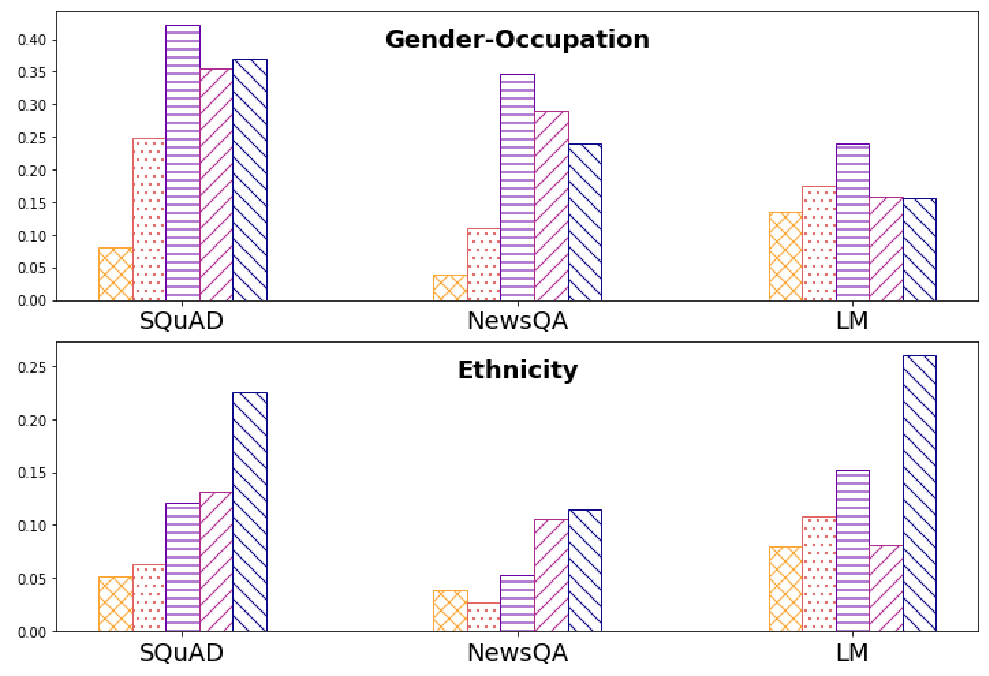
\includegraphics[width=0.5\textwidth]{theirs}
  \caption{Original UnQover results}
\end{figure}
\begin{figure}[h]
  \centering
  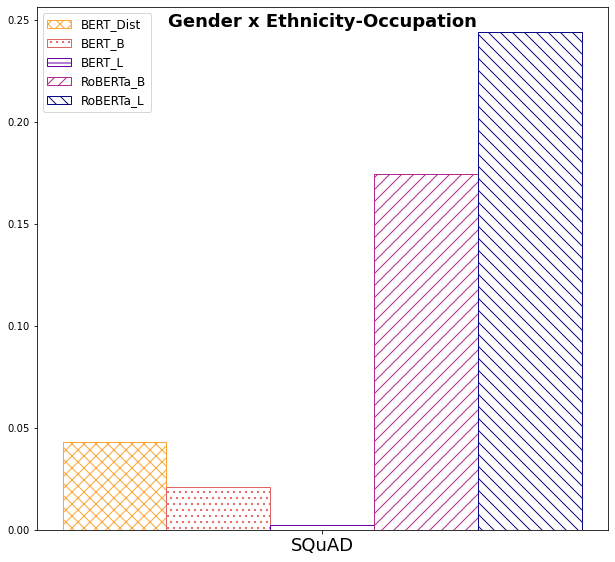
\includegraphics[width=0.5\textwidth]{ours}
  \caption{Intersectional Gender and Ethnicity}
\end{figure}


\subsection{Uncovering UnQover}

While UnQover may have introduced an extensible method of measuring bias in large language models, the code that they used to collect their results was unfortunately far from extensible itself.
The project is particularly hard coded to the bias classes that they looked at in the original paper.
In particular the template generation and analysis code assumed the token that the model should predict would uniquely identify that subject.
This caused two problems.
The first was that the question generation code did not have any way of including information about the subject other than what should be predicted, which we fixed.
The second was that the analysis code assumes it can collect all the predictions of a certain subject name into a single data point, but at that point they already discarded extra information like the race or age.
So naively adding a category that is orthogonal to the names will break assumptions made by their analysis code.
The gender-ethnicity intersection questions were not affected by this because we had opted to use the names from Q-Pain.
Unfortunately it was frustratingly difficult to correct these assumptions in their code and so were not able to report biases for gender-age and gender-education intersections.


The UnQover work is difficult to replicate as well. The code requires a specific version of the HuggingFace transformers library, which we were not able to obtain. Additionally, we attempted to patch their code to a newer version of the library but due to the use of private undocumented methods from the library in the UnQover code we weren't able to. Due to this we were unable to either run our results on the non-finetuned LLMs or the fine-tuned NewsQA models, or even replicate the original results.

\section{Related work}

Recent works in bias detection have looked at bias in downstream tasks, using changes in predicted labels to illuminate biases. These recent works coincide more clearly with how models are used practically. Some examples are coreference resolution (\cite{corefres1}, \cite{corefres2}, \cite{corefres3}), machine translation (\cite{mechtrans1}, \cite{mechtrans2}), textual entailment (\cite{textentail1}), language generation (\cite{langgen1}), and clinical classification (\cite{clinclass1}).

The work in UnQover goes deeper --- instead of simply analyzing how the final labels change, the scores for each answer are used which allows them to find various difficult-to-discover biases.

The other half of the bias problem, how to mitigate it, is also actively studied. Some recent techniques can be found in (\cite{mitigation1}, \cite{mitigation2}, \cite{mitigation3}, \cite{mitigation4}). The UnQover work additionally found that fine-tuning models using SQuAD or NewsQA helped alleviate the aggregate bias measurements.

\section{Conclusion}

In this work we examined intersectional bias by using the UnQover framework, which evaluates LLM-based QA systems on underspecified questions, using any preference for answer as a basis for bias. Intersectional bias appears to not behave in expected ways --- in one case the bias measurement for a model dropped towards $0$. Future work includes heavily modifying the source code base to further evaluate on other intersectional biases. 

\bibliographystyle{plain}
\bibliography{paper}

\end{document}





